\documentclass[12pt]{article}

\usepackage{sbc-template}

\usepackage{graphicx,url}

% \usepackage[brazil]{babel}
\usepackage[latin1]{inputenc}

\sloppy

\title{Proposta de utiliza��o de dados semanticamente estruturados no \textit{software} ``P� na estrada"}

\author{�talo Paiva Batista\inst{1}, Emilie Trindade de Morais\inst{1}}

\address{Faculdade UnB Gama -- Universidade de Bras�lia (UnB)\\
  �rea Especial de Ind�stria Proje��o A -- 72444-240 -- Bras�lia -- DF -- Brazil
  \email{italo.paiva.b@gmail.com, emilie.morais.t@gmail.com}
}

\begin{document} 

\maketitle

\begin{abstract}
  
\end{abstract}
     
\begin{resumo}
  
\end{resumo}

\section{Introdu��o}

\section{Metodologia}

O m�todo escolhido para a constru��o dessa ontologia foi o m�todo \textit{\textbf{Ontology 101}}.

De acordo com \cite{breitman05}, o processo de constru��o de uma ontologia a partir do m�todo 101, resumidamente, 
envolve as seguintes etapas:
  \begin{itemize}
   \item Defini��o das classes dessa ontologia;
   \item Disposi��o das classes em uma hierarquia taxon�mica;
   \item Defini��o de propriedades e valores para os mesmos;
   \item Preenchimento dos valores das propriedades para cada inst�ncia.
  \end{itemize}

Essas quatro etapas resumem os sete passos que podem ser vistos na Figura \ref{fig:processo_101}.
\begin{figure}[ht] 
\centering 
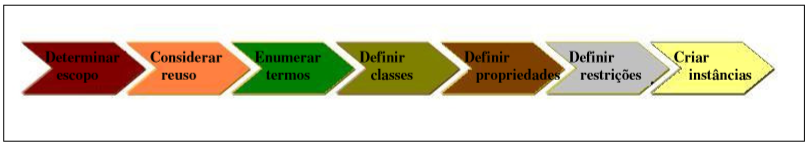
\includegraphics[width=.9\textwidth]{11.png} 
\caption[Processo de desenvolvimento de ontologias.]{Processo de desenvolvimento de ontologias. Fonte: \cite{DanielaLucas2008}}
\label{fig:processo_101}
\end{figure}

Para a considera��o do re�so de ontologias existentes foi realizada uma revis�o de literatura e busca por
ontologias e terminologias j� existentes relacionadas a acidentes e aos dados das
ocorr�ncias no World Wide Web Consortium (W3C). O levantamento das ontologias
foi feito por meio de duas express�es de busca em bases de dados, na
l�ngua inglesa, para obten��o de um resultado mais abrangente.

\begin{center}
  Express�o 1: \textit{Car accident ontology}\\
  Express�o 2: \textit{Traffic accident ontology}
\end{center}


\section{Proposta de modelagem conceitual da ontologia}
  
  \subsection{Escopo da ontologia}
  
  \subsection{Ontologias encontradas}
  
  \subsection{Defini��o das classes}
  
  \subsection{Defini��o das propriedades}
  
\section{Considera��es finais}
  \subsection{Propostas futuras}

% Figure example
% \begin{figure}[ht]
% \centering
% \includegraphics[width=.3\textwidth]{fig2.jpg}
% \caption{This figure is an example of a figure caption taking more than one
%   line and justified considering margins mentioned in Section~\ref{sec:figs}.}
% \label{fig:exampleFig2}
% \end{figure}

% \begin{table}[ht]
% \centering
% \caption{Variables to be considered on the evaluation of interaction
%   techniques}
% \label{tab:exTable1}
% \includegraphics[width=.7\textwidth]{table.jpg}
% \end{table}

\bibliographystyle{sbc}
\bibliography{sbc-template}

\end{document}
